\documentclass[border=6pt]{standalone}
\usepackage{tikz}
\usepackage{pgfplots}
\pgfplotsset{compat=1.18}
\usetikzlibrary{arrows.meta,positioning,shapes.geometric,fit,backgrounds,calc,decorations.pathreplacing,patterns,pgfplots.groupplots}
\tikzset{
  blk/.style={rectangle, rounded corners=2pt, draw=black!70, thick, fill=blue!6,
              minimum height=8mm, minimum width=20mm, align=center, font=\small},
  io/.style={rectangle, rounded corners=6pt, draw=black!70, thick, fill=green!8,
             minimum height=8mm, align=center, font=\small},
  proc/.style={rectangle, draw=black!70, thick, fill=orange!10, minimum height=8mm,
               align=center, font=\small},
  dec/.style={diamond, aspect=2, draw=black!70, thick, fill=yellow!15, align=center, font=\footnotesize},
  warnbox/.style={rectangle, rounded corners=2pt, draw=red!60!black, thick, fill=red!7,
                  minimum height=8mm, align=center, font=\small},
  oklbox/.style={rectangle, rounded corners=2pt, draw=green!45!black, thick, fill=green!8,
                 minimum height=8mm, align=center, font=\small},
  ar/.style={-{Latex[length=2mm]}, thick},
  arl/.style={-{Latex[length=2mm]}, thick, dashed, draw=black!55},
  lbl/.style={font=\footnotesize\itshape, text=black!60},
}
\definecolor{good}{RGB}{34,139,34}
\definecolor{bad}{RGB}{178,34,34}
\definecolor{warn}{RGB}{218,165,32}
\definecolor{pesblue}{RGB}{0,45,98}
\definecolor{complete}{RGB}{30,125,79}
\definecolor{partial}{RGB}{176,106,0}
\definecolor{blocked}{RGB}{166,43,43}
\begin{document}
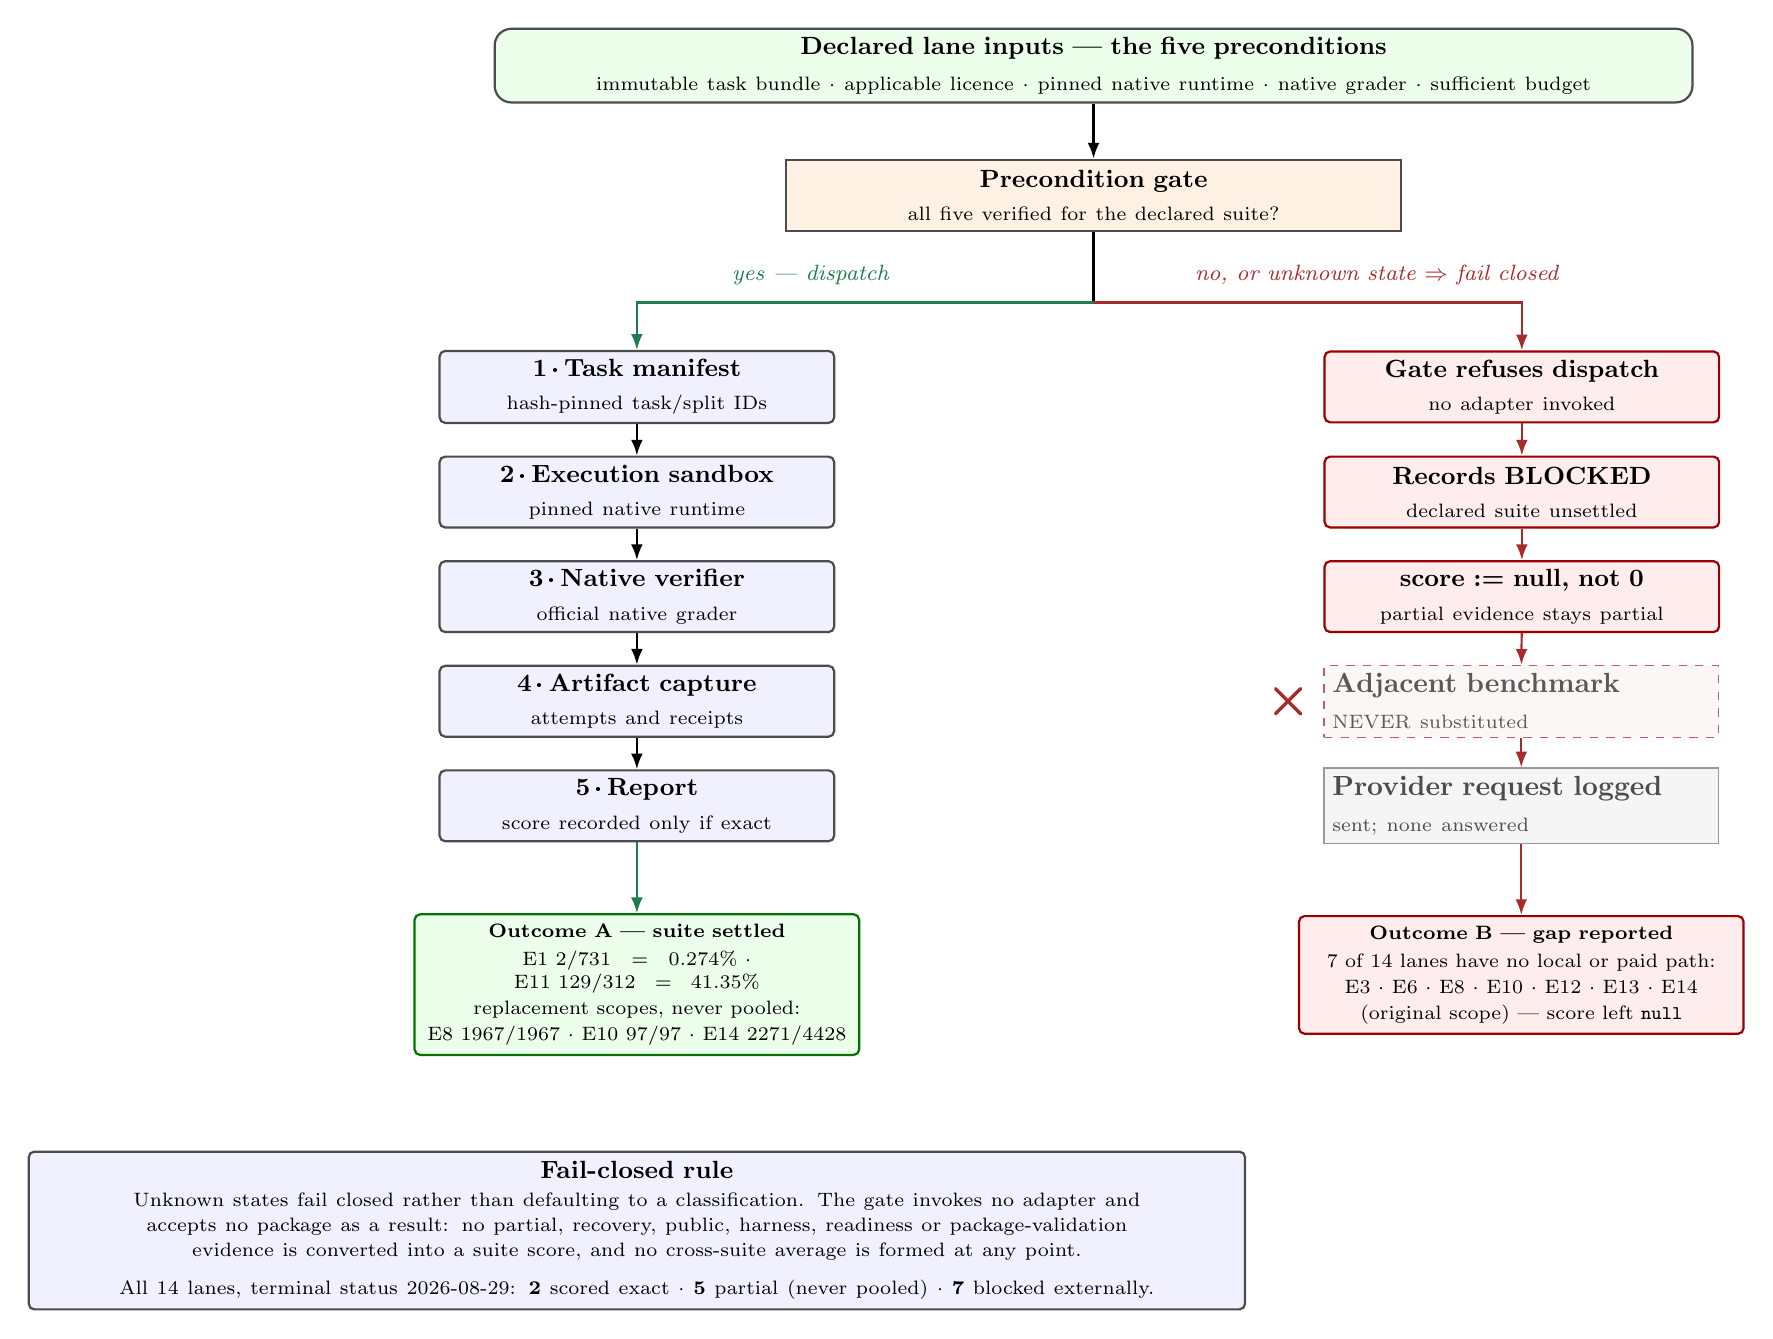
\begin{tikzpicture}[x=1cm,y=1cm]

% ---- local sizing: every box is exactly two lines tall --------------
\tikzset{
  stage/.style={text width=48mm, minimum height=9mm, inner sep=3pt},
  outcome/.style={text width=54mm, minimum height=9mm, inner sep=3.5pt,
                  font=\fontsize{7}{8.3}\selectfont},
  gbox/.style={proc, text width=76mm, minimum height=9mm, inner sep=3pt},
}

% ================= declared inputs =================
\node[io, text width=150mm, minimum height=8.5mm, inner sep=3pt] (spec) at (0,0)
  {\textbf{Declared lane inputs --- the five preconditions}\\[2pt]
   \scriptsize immutable task bundle $\cdot$ applicable licence $\cdot$ pinned native runtime
   $\cdot$ native grader $\cdot$ sufficient budget};

% ================= precondition gate =================
\node[gbox, below=7mm of spec] (g)
  {\textbf{Precondition gate}\\[1pt]
   \scriptsize all five verified for the declared suite?};

\draw[ar] (spec) -- (g);

% ================= split into the two outcomes =================
\draw[thick] (g.south) -- ++(0,-9mm) coordinate (mid);
\coordinate (xL) at (-5.8,0);
\coordinate (xR) at ( 5.8,0);
\coordinate (splitL) at (xL |- mid);
\coordinate (splitR) at (xR |- mid);

\node[lbl, text=complete, anchor=south] at ($(mid)!0.62!(splitL)+(0,1mm)$)
  {yes --- dispatch};
\node[lbl, text=blocked, anchor=south] at ($(mid)!0.62!(splitR)+(0,1mm)$)
  {no, or unknown state $\Rightarrow$ fail closed};

% ================= LEFT: preconditions satisfied =================
\node[blk, stage] (l1) [below=6mm of splitL]
  {\textbf{1\,\textperiodcentered\,Task manifest}\\[1pt] \scriptsize hash-pinned task/split IDs};
\node[blk, stage, below=4mm of l1] (l2)
  {\textbf{2\,\textperiodcentered\,Execution sandbox}\\[1pt] \scriptsize pinned native runtime};
\node[blk, stage, below=4mm of l2] (l3)
  {\textbf{3\,\textperiodcentered\,Native verifier}\\[1pt] \scriptsize official native grader};
\node[blk, stage, below=4mm of l3] (l4)
  {\textbf{4\,\textperiodcentered\,Artifact capture}\\[1pt] \scriptsize attempts and receipts};
\node[blk, stage, below=4mm of l4] (l5)
  {\textbf{5\,\textperiodcentered\,Report}\\[1pt] \scriptsize score recorded only if exact};

\foreach \a/\b in {l1/l2, l2/l3, l3/l4, l4/l5} {\draw[ar] (\a) -- (\b);}
\draw[ar, draw=complete] (mid) -| (l1);

% ================= RIGHT: fail-closed branch =================
\node[warnbox, stage, right=62mm of l1] (r1)
  {\textbf{Gate refuses dispatch}\\[1pt] \scriptsize no adapter invoked};
\node[warnbox, stage, right=62mm of l2] (r2)
  {\textbf{Records BLOCKED}\\[1pt] \scriptsize declared suite unsettled};
\node[warnbox, stage, right=62mm of l3] (r3)
  {\textbf{score := null, not 0}\\[1pt] \scriptsize partial evidence stays partial};
\node[stage, draw=blocked!75, dashed, fill=blocked!4, text=black!65, right=62mm of l4] (r4)
  {\textbf{Adjacent benchmark}\\[1pt] \scriptsize NEVER substituted};
\node[stage, draw=black!40, fill=black!4, text=black!70, right=62mm of l5] (r5)
  {\textbf{Provider request logged}\\[1pt] \scriptsize sent; none answered};

\foreach \a/\b in {r1/r2, r2/r3, r3/r4, r4/r5} {\draw[ar, draw=blocked] (\a) -- (\b);}
\draw[ar, draw=blocked] (mid) -| (r1);

% cross marking the refusal to substitute an adjacent benchmark
\coordinate (xk) at ($(r4.west)+(-0.45,0)$);
\draw[blocked, very thick, line cap=round] ($(xk)+(-0.16,0.16)$) -- ($(xk)+(0.16,-0.16)$);
\draw[blocked, very thick, line cap=round] ($(xk)+(-0.16,-0.16)$) -- ($(xk)+(0.16,0.16)$);

% ================= the two outcomes, side by side =================
\node[oklbox, outcome, below=9mm of l5] (oa)
  {\textbf{Outcome A --- suite settled}\\[2pt]
   E1 $2/731 = 0.274\%$ $\cdot$ E11 $129/312 = 41.35\%$\\[1pt]
   replacement scopes, never pooled:\\[1pt]
   E8 $1967/1967$ $\cdot$ E10 $97/97$ $\cdot$ E14 $2271/4428$};
\draw[ar, draw=complete] (l5) -- (oa);

\node[warnbox, outcome, below=9mm of r5] (ob)
  {\textbf{Outcome B --- gap reported}\\[2pt]
   7 of 14 lanes have no local or paid path:\\[1pt]
   E3 $\cdot$ E6 $\cdot$ E8 $\cdot$ E10 $\cdot$ E12 $\cdot$ E13 $\cdot$ E14\\[1pt]
   (original scope) --- score left \texttt{null}};
\draw[ar, draw=blocked] (r5) -- (ob);

% ================= closing rule strip =================
\node[blk, text width=152mm, inner sep=3.5pt, below=12mm of oa]
  {\textbf{Fail-closed rule}\\[2pt]
   \scriptsize Unknown states fail closed rather than defaulting to a classification. The gate invokes no adapter and\\[1pt]
   \scriptsize accepts no package as a result: no partial, recovery, public, harness, readiness or package-validation\\[1pt]
   \scriptsize evidence is converted into a suite score, and no cross-suite average is formed at any point.\\[3pt]
   \scriptsize All 14 lanes, terminal status 2026-08-29: \textbf{2} scored exact $\cdot$ \textbf{5} partial (never pooled) $\cdot$ \textbf{7} blocked externally.};

\end{tikzpicture}
\end{document}
